
\documentclass{beamer}


\mode<presentation>
{
  \usetheme{Hawke}
  \setbeamercovered{transparent}
}


\usepackage[english]{babel}
\usepackage[latin1]{inputenc}
\usepackage{times}
\usepackage[T1]{fontenc}
\usepackage{multimedia}
\usepackage{mathtools}

\title[Lecture 1]{Lecture 1 - Introduction}

\author[I. Hawke]{I.~Hawke}

\institute[University of Southampton]
{
  School of Mathematics, \\
  University of Southampton, UK
}

\date[Semester 1]{MATH3018/6141, Semester 1}

\subject{Numerical methods}

\pgfdeclareimage[height=0.5cm]{university-logo}{mathematics_7469}
\logo{\pgfuseimage{university-logo}}

\AtBeginSection[]
{
  \begin{frame}<beamer>
    \frametitle{Outline}
    \tableofcontents[currentsection]
  \end{frame}
}


\begin{document}

\begin{frame}
  \titlepage
\end{frame}

\section{Numerical methods - introduction}

\subsection{What are numerical methods?}

\begin{frame}
  \frametitle{Examples}

  \begin{overlayarea}{\textwidth}{0.8\textheight}
    \only<1|handout:1>
    {
      \begin{center}

        \vspace{2ex}
        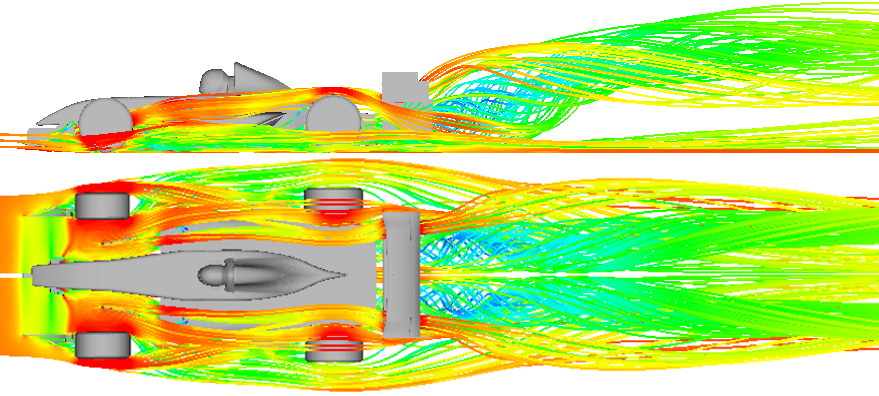
\includegraphics[width=0.95\textwidth]{figures/Kenji_Glue_Crop3}
        \vspace{3ex}

        Computing air flow past complex shapes {\tiny [MSc Race Car
          Aerodynamics students, School of Engineering Sciences]}.
      \end{center}
    }
    \only<2|handout:2>
    {
      \begin{center}
        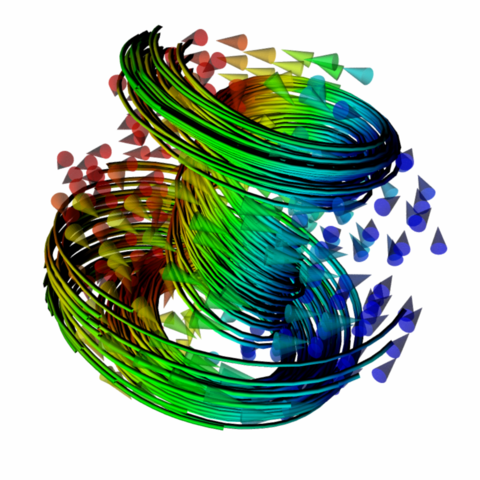
\includegraphics[width=0.6\textwidth]{figures/0mT_zeeman_Fangohr_Ferromagnetic_Sphere}

        Complex magnetic field structures \href{http://www.soton.ac.uk/~rpb/thesis.pdf}{\tiny [Boardman \& Fangohr]}.
      \end{center}
    }
    \only<3|handout:3>
    {
      \begin{center}
        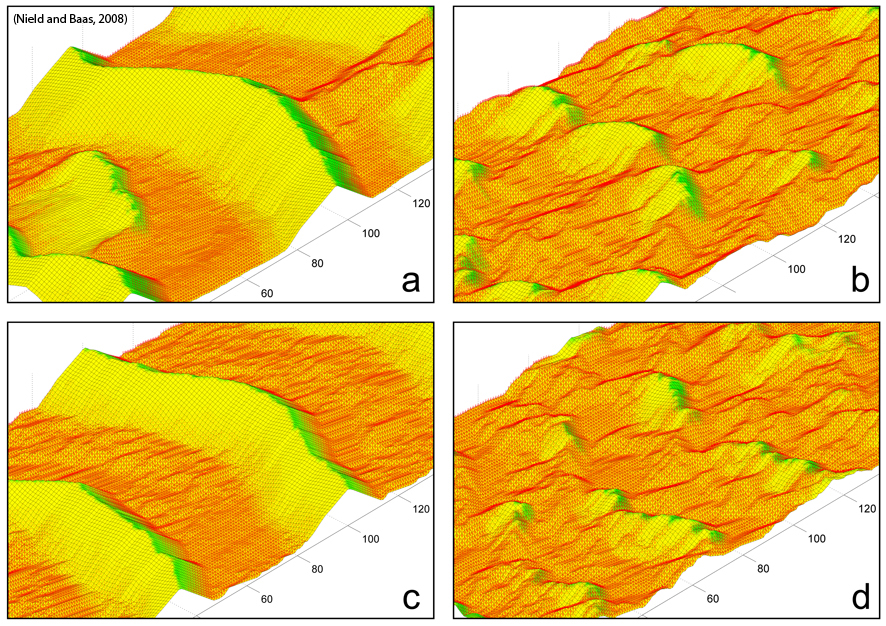
\includegraphics[width=0.8\textwidth]{figures/3d_landscape_samples_NieldDunes}

        Geographical modelling {\tiny
          \href{http://dx.doi.org/10.1016/j.gloplacha.2008.10.002}{[Nield \&
            Baas, Global and Planetary Change 64 (2008)]}}.
      \end{center}
    }
    \only<4|handout:4>
    {
      \begin{center}
        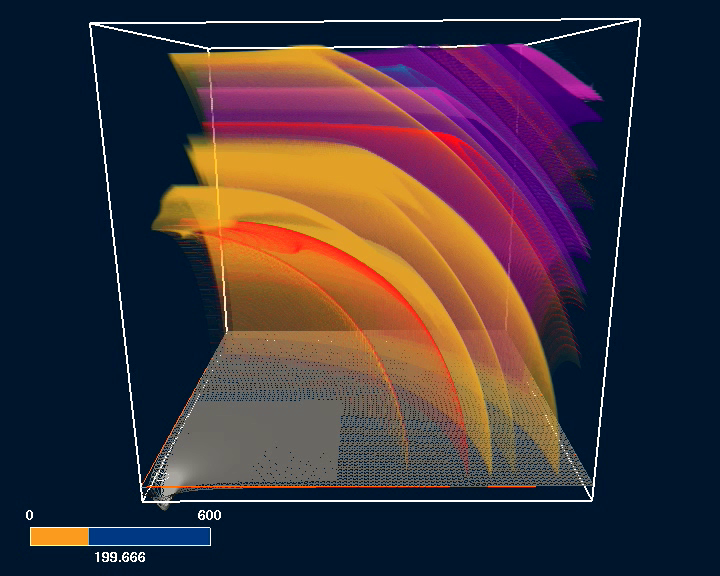
\includegraphics[width=0.67\textwidth]{figures/collapse6}

        Computing gravitational waves emitted in neutron star collapse
        to black hole
        \href{http://dx.doi.org/10.1088/0264-9381/24/12/S13}{{\tiny
            [Baiotti, Hawke, Rezzolla, Schnetter; K{\"a}hler]}}.
      \end{center}
    }
    \only<5|handout:5>
    {
      \begin{center}
        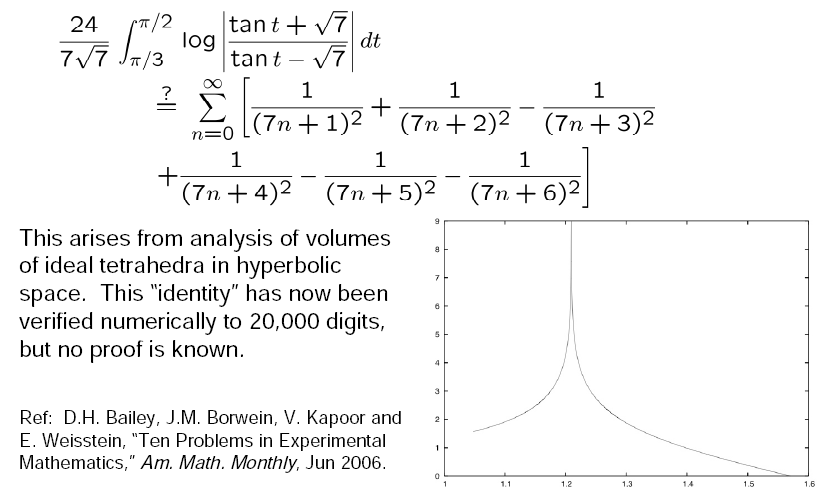
\includegraphics[width=0.95\textwidth]{figures/QuadPic1}

        Suggesting and testing purely mathematical results.
      \end{center}
    }
  \end{overlayarea}

\end{frame}

\begin{frame}
  \frametitle{What are numerical methods?}

  \begin{quotation}
    Numerical methods are algorithms that give quantitative answers in
    a finite number of steps.
  \end{quotation}
  \pause
  \begin{itemize}
  \item Problem \emph{continuous} (eg
    differential equation) implies answer is  approximate.\pause
  \item Usefulness of algorithm is practically defined by the
    number of steps to find answer at given accuracy.\pause
  \item In particular: \emph{useless}
    algorithms exist - more steps need not improve accuracy.
  \end{itemize}

\end{frame}


\begin{frame}
  \frametitle{Where do numerical methods fit?}

  \begin{center}
    \includegraphics[width=0.9\textwidth]{figures/ModelMethodReality}
  \end{center}

\end{frame}


\subsection{What is this course?}

\begin{frame}
  \frametitle{What is this course?}

  This course aims to introduce three areas of numerical methods.\pause

  \begin{enumerate}
  \item<2-> How are specific algorithms implemented?
    \begin{itemize}
    \item ``Engineering'' aspect.
    \item Practical implementation using Python.
    \item Class test (10\%) and coursework (30\%).
    \end{itemize}
  \item<3-> How efficient are the algorithms and how can they be
    implemented efficiently?
    \begin{itemize}
    \item ``Computer science'' aspect.
    \item Mixture of analytic and practical, Python work.
    \item Mainly coursework (30\%).
    \end{itemize}
  \item<4> How do we derive algorithms and prove that they work?
    \begin{itemize}
    \item ``Mathematics'' aspect.
    \item Analytic, but feeds into practical work.
    \item Closed book exam (60\%).
    \end{itemize}
  \end{enumerate}

\end{frame}


\begin{frame}
  \frametitle{How to think}

  \begin{itemize}
  \item Course will \emph{not} introduce cutting edge
    numerical methods.
  \item Shows how numerical methods are derived and
    analyzed. \pause
  \item Course notes contain the formal material that
    might be examined.
  \item Lectures illustrate by example how the algorithms are understood,
    implemented and used. \pause
  \item Computer labs  introduce Python needed to
    illustrate and implement the algorithms.
  \end{itemize}

\end{frame}


\section{Approximation pitfalls}


\subsection{Finite precision}


\begin{frame}
  \frametitle{Finite precision and approximation}

  Most numerical algorithms involve real numbers. Computer
  representations in \emph{floating point} notation are
  approximations:
  \begin{equation*}
    \pi \rightarrow 0.\underbracket{314159265358979}_{\text{precision}} \times 10^{\overbracket{1}^{\text{\clap{exponent}}}}.
  \end{equation*}
  Precision of representation -- number of significant
  digits -- controls accuracy: can never be perfect.

\end{frame}


\begin{frame}
  \frametitle{$1 + 1 = \dots$}

  Imagine a computer with 1 digit of precision. It
  represents $1$ and $0.1$ exactly. It also represents
  \begin{equation*}
    1 + 1 = 2
  \end{equation*}
  precisely. \pause

  Computer cannot represent sum of $1$ and $0.1$:
  \begin{align*}
    1 + 0.1 & = 1.1 \\
            & = 0.11 \times 10^1 \\
            & \rightarrow 0.1 \times 10^1 \\
            & = 1
  \end{align*}

\end{frame}


\begin{frame}
  \frametitle{$1 + 1 = 2$?}

  On a computer with a single digit of precision,
  \begin{align*}
    1 + \sum_1^{10} 0.1 & = (1 + 0.1) + 0.1 + \dots 0.1 \\
                        & = \dots \\
                        & = 1
  \end{align*} \pause
  \emph{or}
  \begin{align*}
    1 + \sum_1^{10} 0.1 & = 1 + (0.1 + \dots 0.1) \\
                        & = 1 + 1 \\
                        & = 2.
  \end{align*}

\end{frame}

\begin{frame}
  \frametitle{Matrix problems}

  Many numerical methods depend on solving linear systems. Consider
  \begin{equation*}
    \begin{pmatrix}
      4 & 5 \\ 2 & 3
    \end{pmatrix} {\bf x} = {\bf b}.
  \end{equation*}
  This is a sensible matrix equation. \pause

  Problem has solution if (and only if) matrix is
  non-singular:
  \begin{equation*}
    \det (A) = 4 \times 3 - 5 \times 2 = 2 \neq 0,
  \end{equation*}
  so problem has a solution. \pause
%
  \emph{However}, with only one digit of precision
  \begin{align*}
    \det (A) & = 4 \times 3 - 5 \times 2 && = (12) - (10) \\
             &&& \rightarrow (10) - (10)  = 0.
  \end{align*} \pause
  Finite precision makes matrix singular; no solution can be
  found!

\end{frame}

\subsection{Summary}

\begin{frame}
  \frametitle{Summary}

  \begin{itemize}
  \item Numerical methods are about computing quantitative answers
    using a finite number of steps.
  \item The finite accuracy of numerical methods leads to inherent
    approximations.
  \item These approximations can lead to fundamental mathematical
    difficulties.
  \end{itemize}

\end{frame}

\end{document}
